\documentclass[11pt]{article}

\usepackage[a4paper,margin=1in]{geometry}
\usepackage{amsmath}
\usepackage{booktabs}
\usepackage{tikz}
\usepackage{hyperref}

\title{Rig Geometry: PRO4500 Projector Distance\\ and Telecentric Camera Angle}
\author{Micro-Projection}
\date{\today}

\begin{document}
\maketitle

\section{Setup}

The projector illuminates a flat surface at (approximately) normal incidence,
aimed at a center point $O$. A telecentric-lens camera is also aimed at $O$,
with its optical axis tilted by an angle $\theta$ away from the surface
normal (Figure~\ref{fig:setup}). Because the camera's lens is telecentric,
its imaging cone is a bundle of parallel rays with a fixed rectangular
cross-section $W_0 \times H_0$ --- unlike a normal lens, this cross-section
does not change with working distance. Tilting the camera changes how that
fixed cross-section intersects the (untilted) surface plane.

\begin{figure}[h]
\centering
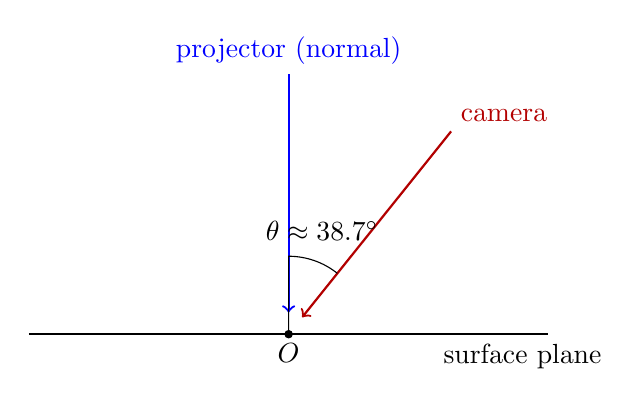
\begin{tikzpicture}[scale=1.1]
  \draw[thick] (-3,0) -- (3,0);
  \node[below] at (2.7,0) {surface plane};
  \filldraw (0,0) circle (1.2pt) node[below] {$O$};

  \draw[->, thick, blue] (90:3) -- (90:0.25);
  \node[blue, above] at (90:3) {projector (normal)};

  \draw[->, thick, red!70!black] (51.3:3) -- (51.3:0.25);
  \node[red!70!black, above right] at (51.3:3) {camera};

  \draw (0,0) -- (90:0.9) arc[start angle=90, end angle=51.3, radius=0.9];
  \node at (72:1.25) {$\theta \approx 38.7^\circ$};
\end{tikzpicture}
\caption{Side-view schematic in the tilt plane: projector at normal
incidence, camera tilted by $\theta$, both aimed at the surface center
$O$.}
\label{fig:setup}
\end{figure}

Two questions follow from this geometry:
\begin{enumerate}
  \item At what working distance $D$ does the projector produce an image
        whose \emph{height} equals the camera's fixed capturable height
        $H_0$?
  \item At what tilt angle $\theta$ does the camera's covered
        \emph{width} expand to match the projector's image width at that
        distance?
\end{enumerate}

\section{Confirmed hardware}

\begin{table}[h]
\centering
\begin{tabular}{@{}lll@{}}
\toprule
Component & Key parameters & Source \\
\midrule
Wintech PRO4500 & 460\,nm LED, 700\,mm lens & Wintech PRO4500 \\
(3D-measurement config.) & $D_0 = 700$\,mm, FOV $400\times250$\,mm & brochure \\
 & projected pixel $305\,\mu$m & \\[2pt]
FLIR Blackfly S & ON Semi PYTHON 1300 CMOS & FLIR / Edmund \\
BFS-U3-13Y3M-C & $1280\times1024$\,px, $4.8\,\mu$m pitch & Optics datasheets \\
 & sensing area $6.14\times4.92$\,mm & \\[2pt]
Edmund Optics 0.09X & magnification $M=0.09\times$ & Edmund Optics \\
$\tfrac{1}{2}''$ GoldTL & focusable WD $132$--$182$\,mm & \#58-259 (15171) \\
telecentric lens & max sensor format $\tfrac{1}{2}''$ & \\
\bottomrule
\end{tabular}
\caption{Hardware specifications used below. The PRO4500's other
lens/LED options (92/184\,mm working distance, $65.6{\times}41$ /
$131.2{\times}82$\,mm FOV) belong to a different, lower-quality projector
and are not used here.}
\end{table}

\section{Camera's fixed field of view}

A telecentric lens holds magnification $M$ constant across its focus
range, so the object-side field of view is simply the sensor size divided
by $M$:
\begin{equation}
  W_0 = \frac{w_{\text{sensor}}}{M}, \qquad
  H_0 = \frac{h_{\text{sensor}}}{M}.
\end{equation}
With $w_{\text{sensor}} = 6.14$\,mm, $h_{\text{sensor}} = 4.92$\,mm,
$M = 0.09$:
\begin{equation}
  W_0 = \frac{6.14}{0.09} = 68.22\text{\,mm}, \qquad
  H_0 = \frac{4.92}{0.09} = 54.67\text{\,mm}.
\end{equation}
This footprint is fixed anywhere in the lens's $132$--$182$\,mm focus
range; where exactly the camera sits within that range is a free choice
that does not affect $W_0, H_0$.

\section{Projector image size vs.\ working distance}

For a fixed projection lens, image size scales linearly with throw
distance (similar triangles about the lens's exit pupil). Using the
PRO4500's rated point $(D_0, H_{\text{proj},0}) = (700, 250)$\,mm as the
calibration point:
\begin{equation}
  H_{\text{proj}}(D) = D \cdot \frac{250}{700} = D \cdot \frac{5}{14},
  \qquad
  W_{\text{proj}}(D) = D \cdot \frac{400}{700} = D \cdot \frac{4}{7}.
\end{equation}
Both preserve the PRO4500's fixed image aspect ratio
$400/250 = 1.6$.

\section{Matching distance \texorpdfstring{$D$}{D}}

Set $H_{\text{proj}}(D) = H_0$:
\begin{equation}
  D = H_0 \cdot \frac{14}{5} = 54.67 \times 2.8 \approx 153.1\text{\,mm}.
\end{equation}
At this distance the projector's image is
\begin{equation}
  W_{\text{proj}}(D) = H_0 \times 1.6 = 54.67 \times 1.6 \approx 87.47\text{\,mm}
\end{equation}
wide, by $H_0 = 54.67$\,mm tall --- matching the camera's height exactly.

\section{Telecentric footprint under an oblique view}

A telecentric lens's imaging cone is a bundle of parallel rays with
cross-section $W_0 \times H_0$, measured in the plane perpendicular to the
camera's optical axis. Tilting that axis by $\theta$ from the surface
normal is equivalent to a beam of width $W_0$ striking a plane at
incidence angle $\theta$: the illuminated footprint stretches by
$1/\cos\theta$ along the tilt direction, while the dimension
perpendicular to the tilt (here, height) is unchanged:
\begin{equation}
  W(\theta) = \frac{W_0}{\cos\theta}, \qquad H(\theta) = H_0.
\end{equation}

\section{Solving for \texorpdfstring{$\theta$}{theta}}

Require the camera's tilted width to cover the projector's image width at
the matching distance $D$:
\begin{equation}
  \frac{W_0}{\cos\theta} = W_{\text{proj}}(D) = 1.6\, H_0
  \quad\Longrightarrow\quad
  \cos\theta = \frac{W_0 / H_0}{1.6}.
\end{equation}
Notably, $W_0/H_0 = w_{\text{sensor}}/h_{\text{sensor}}$ --- the
magnification $M$ (and hence the absolute field-of-view scale) cancels
out. The required tilt depends only on the sensor's aspect ratio and the
projector's image aspect ratio:
\begin{equation}
  \cos\theta = \frac{6.14/4.92}{1.6} = \frac{1.2480}{1.6} = 0.7800
  \quad\Longrightarrow\quad
  \theta \approx 38.7^\circ.
\end{equation}

\section{Results}

\begin{table}[h]
\centering
\begin{tabular}{@{}lr@{}}
\toprule
Quantity & Value \\
\midrule
Camera FOV, square-on ($W_0 \times H_0$) & $68.22 \times 54.67$\,mm \\
Camera working distance (free choice) & $132$--$182$\,mm \\
Projector working distance $D$ & $\approx 153.1$\,mm \\
Projector image at $D$ & $87.47 \times 54.67$\,mm \\
\textbf{Camera tilt angle $\theta$} & $\approx 38.7^\circ$ \\
Covered surface & $87.47 \times 54.67$\,mm \\
\bottomrule
\end{tabular}
\end{table}

\section{Caveats}

\begin{itemize}
  \item The projector's image-size-vs-distance law is a first-order
        (thin-lens, linear) approximation calibrated on a single
        datasheet point ($700$\,mm); the brochure does not document a
        focus range for the $700$\,mm lens, so operating it at
        $153$\,mm assumes it can be refocused that far from its nominal
        point.
  \item The telecentric lens is assumed to fill the sensor format
        uniformly in both axes, i.e.\ FOV aspect ratio equals sensor
        aspect ratio.
  \item At $\theta \approx 38.7^\circ$, points across the tilted
        footprint sit at different distances along the camera's optical
        axis; a Scheimpflug-adjusted mount (or reliance on the lens's
        $\pm 63.6$\,mm depth of field at $f/10$) is needed to keep the
        whole footprint in focus.
\end{itemize}

\end{document}
